% Document class, language and encoding setup
\documentclass[a4paper,12pt,english]{report}

\usepackage[english]{babel}
\usepackage[utf8]{inputenc}
\usepackage[T1]{fontenc}
% Fixing the font issue
\usepackage{ae,aecompl}

% Color package
\PassOptionsToPackage{dvipsnames}{xcolor}
	\RequirePackage{xcolor} % [dvipsnames] 
	
% Allows page-links in pdf file
\usepackage{hyperref}
\hypersetup{
% Uncomment the line below to remove all links (to references, figures, tables, etc)
%draft, 
%colorlinks=true, linktocpage=true, pdfstartpage=3, pdfstartview=FitV,
% Uncomment the line below if you want to have black links (e.g. for printing black and white)
colorlinks=true, linktocpage=true, pdfborder={0 0 0}, 
pdfstartpage=3, pdfstartview=FitV, hypertexnames=true, pdfhighlight=/O, 
breaklinks=true, pdfpagemode=UseNone, pageanchor=true, pdfpagemode=UseOutlines, plainpages=false,
bookmarksnumbered, bookmarksopen=true, bookmarksopenlevel=1,
urlcolor=Black, linkcolor=Black, citecolor=Black,
%------------------------------------------------
% PDF file meta-information
%pdftitle={\myTitle},
%pdfauthor={\textcopyright\ \myName, \myUni, \myFaculty},
%pdfsubject={},
%pdfkeywords={},
%pdfcreator={pdfLaTeX},
%pdfproducer={LaTeX with hyperref and classicthesis}
%------------------------------------------------
} 

\usepackage{pdfpages}
% Todo notes package and commands
\usepackage{todonotes}
% Allows commands to emit a space "at the end"
\usepackage{xspace}
%tabularextension
\usepackage{longtable}
% Listings setup
\usepackage{listings}

% Graphics setup
\usepackage{graphicx}
\graphicspath{{./graphics/} {./graphics/sprint1/}}

\usepackage{tikz}
\usetikzlibrary{calc}
\usetikzlibrary{arrows,backgrounds,snakes}

\usepackage{tikz-uml}

\usepackage{amsmath}
\usepackage{amssymb}

% Advanced tables
\usepackage{tabularx}
\usepackage{multirow}

% Clever references
\usepackage{cleveref}

% Named references
\usepackage{nameref}

% Bibliography
\usepackage[square,numbers]{natbib}
\bibliographystyle{unsrt}

% Force position [H]
\usepackage{float}

% For figures with sub-figures
\usepackage{subcaption}

% Caption package. Makes label of caption bold.
\usepackage[labelfont=bf]{caption}

% Additional commands
\newcommand{\namedtodo}[5]
{
  \ifthenelse{\equal{#1}{}}
  {
    \todo[backgroundcolor=#4,caption=
    {\textbf{#3: } #2}
    ,inline]
    {\color{#5}\textbf{#3: }#2}
  }
  {
    \todo[backgroundcolor=#4,caption=
    {\textbf{#3: } #1}
    ,inline]
    {\color{#5}\textbf{#3: }#2}
  }
}
\newcommand{\mikkel}[2][]{\namedtodo{#1}{#2}{Mikkel}{blue!80}{white}}
\newcommand{\stefan}[2][]{\namedtodo{#1}{#2}{Stefan M}{orange}{black}}
\newcommand{\anders}[2][]{\namedtodo{#1}{#2}{Anders}{orange}{black}}
\newcommand{\thilemann}[2][]{\namedtodo{#1}{#2}{Stefan T}{NavyBlue!35}{NavyBlue}}
\newcommand{\mikael}[2][]{\namedtodo{#1}{#2}{Mikael}{green}{black}}
\newcommand{\bruno}[2][]{\namedtodo{#1}{#2}{Bruno}{black!10!red!90}{white}}
% Her er en liste over navnene på de forskellige styles
% C#: csharp
% F#: fsharp

% 
% Listings kan refereres vha. \cref{}
\crefname{listing}{code example}{code example}
\Crefname{listing}{Code example}{code examples}
% 

%Algoritmer i cref
\crefname{algocf}{algorithm}{algorithm}
\Crefname{algocf}{Algorithm}{Algorithms}
%

% Angivelse af navn på listings
\renewcommand\lstlistingname{Code example}
\renewcommand\lstlistlistingname{Code example}

\lstdefinestyle{standard}
{
	frame=shadowbox,
	framesep=5pt,
	rulecolor=\color{blue!40!black},
	rulesepcolor=\color{white!93!black},
	numbers=left,
	basicstyle=\ttfamily,
	numberstyle=\tiny,
	numberfirstline=true,
	%numberblanklines=false,
	stepnumber=1,
	numbersep=9pt,	
	captionpos=b,
	escapeinside={(*}{*)},
	breaklines=true,
	tabsize=4,
	language=c
}

\lstset{style=standard}

\lstdefinestyle{c}
{
	style=standard
}

\lstdefinestyle{csmall}
{
	style=c
}

\lstdefinestyle{csharp}
{
	style=standard,
	language=[Sharp]C
}
\lstdefinestyle{csharpsmall}
{
	style=csharp
}
\lstdefinestyle{fsharp}
{
	language=[Sharp]F,
	frame=lr,
	rulecolor=\color{blue!80!black}
}
\lstdefinestyle{fsharpsmall}
{
	style=fsharp,
	basicstyle=\ttfamily\footnotesize
}


%Definitions
\newcommand{\mindsqualls}{MindSqualls\xspace}
\newcommand{\csharp}{\textsc{C\#}\xspace}
\newcommand{\fsharp}{\textsc{F\#}\xspace}
\newcommand{\legoms}{Lego Mindstorms\xspace}
%\newcommand{\lego}{\textsc{LEGO$^{\textrm{\scriptsize\textregistered}}$}\xspace}
\newcommand{\lego}{Lego\xspace}
\newcommand{\legos}{Legos\xspace}
\newcommand{\kinect}{Kinect\xspace}

%Superscript and subscript
\newcommand{\superscript}[1]{\ensuremath{^{\textrm{#1}}}}
\newcommand{\subscript}[1]{\ensuremath{_{\textrm{#1}}}}

% Degrees
\newcommand{\degree}{\ensuremath{^\circ}}
\newcommand{\dg}{\degree}

\newcommand{\quoter}[1]%
{
  \par
  \vspace{1.5em}
  \addtolength{\leftskip}{1.5cm}
  \addtolength{\rightskip}{1.5cm}
  \textit{#1}
  \addtolength{\leftskip}{-1.5cm}
  \addtolength{\rightskip}{-1.5cm}
  \vspace{1.5em}
  \par
}

% For fancy pseudocode algoritms
\usepackage[algochapter,lined,boxed,noend]{algorithm2e}
\renewcommand{\listalgorithmcfname}{Liste over Algoritmer}
\renewcommand{\algorithmcfname}{Algoritme}
\renewcommand{\algorithmautorefname}{algoritme}
\renewcommand{\algorithmcflinename}{linje}

% Math proofs and stuff.
\usepackage{amsthm}
\usepackage{bigints}

\newcommand{\HRule}{\rule{\linewidth}{0.5mm}}
\begin{document}
%Front page
\begin{titlepage}

\begin{center}

\HRule \\[0.5cm]
\textsc{ \Huge Cars Audio Game}\\

\HRule \\[1cm]

\textsc{\Large SW613F14} \\[2cm]

%picture

\vfill
{\Large Developing Complex Software Systems}
\\ ~\\
{\large Spring Semester 2014}

\end{center}
\end{titlepage}

\pagenumbering{Roman}

\clearpage

\thispagestyle{empty}
\begin{titlepage}
\begin{nopagebreak}
{\samepage 
\begin{tabular}{r}
	\parbox{16cm}{\raisebox{11mm}{
\includegraphics[height=1.2cm]{aauLogoEn.jpg}}
	\hfill \parbox{7cm}{\begin{tabular}{l}
		{\small \textbf{Department of Computer Science}}\\
		{\small Selma Lagerløfs Vej 300} \\
		{\small 9220 Aalborg Ø} \\
		{\small Phone (+45) 9940 9940} \\
		{\small Fax (+45) 9940 9798} \\
		{\small http://cs.aau.dk}
	\end{tabular}}
	}
\end{tabular}

\begin{tabular}{cc}
	\parbox{8cm}{
	\begin{description}
		\item { \textbf{Title:}}\\ 
			Cars Audio Game
    		\item { \textbf{Subject:}}\\ 
			\raggedright Developing Complex Software Systems
	\end{description}
	
	\parbox{8cm}{
	\begin{description}
		\item { \textbf{Project period:}}\\
			03-02-2014 -\\
			28-05-2014
 		\hspace{4cm}
		\item { \textbf{Project group:}}\\
  			sw613f1f
 		\hspace{4cm}
		\item {\textbf{Participants:}}\\
			Bruno Thalmann\\
			Mikael E. Christensen\\
			Mikkel S. Larsen\\
			Stefan M. G. Micheelsen\\
		\hspace{2cm}
		\item { \textbf{Supervisor:}}\\
 			Thomas Pedersen\\
  	\end{description}
	}
	\begin{description}
		\item { \textbf{Printings:} X}
		\item { \textbf{Pages:} X } 
		\item { \textbf{Appendices:} X}
		\item { \textbf{Total pages:} X }
		\item { \textbf{Source code:} X}
	\end{description}
	\vfill } &
	\parbox{6.5cm}{
 	 \vspace{.15cm}
  	\hfill 
  	\begin{tabular}{l}
  		{ Abstract:}\bigskip \\
  		\fbox{
  		\parbox{6cm}{\bigskip
     		{\vfill{\small This project is a part of a multi-project, consisting of 16 groups, from Software-Engineering 6th semester at Aalborg University.
The purpose of the multi-project is to develop a series of applications for autistic people.

The focus of the project-group is a game that should help in improving the auditory sense.
In the game you must control a car, moving from the left to the right, while avoiding or collecting objects.
The car is manoeuvred up and down by the volume of the speech produced by the player.

A speech therapist and two pedagogues from Aalborg Kommune are the main stakeholders of this product.
Throughout the project there has been meeting with the customers to match expectations and manufacture requirements.

To contribute to the multi-project process, the report also contains two chapters to be used by future multi-projects. The first chapter contains a description of the generic framework used to develop the game.
The second chapter is about the git usage in the multi-project, with a detailed explanation of the usage and common mistakes.
     		\bigskip}}
     	}}
   	\end{tabular}}
\end{tabular}
}%samepage end
\\
\vfill
\noindent{\footnotesize{\textit{The content of this report is freely available, but if published it has to be acknowledged by
the authors.}}}
\end{nopagebreak}
\end{titlepage}
\clearpage

\setcounter{page}{4}
\setcounter{secnumdepth}{3}

\newcommand{\prefaceHeaderName}{Preface}
\section*{\prefaceHeaderName}
This report has been made by 6th semester Software-Engineering students at Aalborg University, during the spring-semester of 2014.
It is expected of the reader to have a background in IT/software, due to the technical content.

References and citations are done by the use of numeric notation, e.g. \cite{music-and-computers}, which refers to the first item in the bibliography.
Whenever the report refers to 'we', it is to be understood as the members of the project-group.

On the following page, a glossary can be found, containing words and terms that might not be apparent from their context when used in the report.

We would like to thank our lecturers, as well as our supervisor Thomas Pedersen, for his guidance throughout the semester.

\clearpage

%Table of content
\pdfbookmark{\contentsname}{toc}
\setcounter{tocdepth}{1}
\tableofcontents

\clearpage

\pagenumbering{arabic}

\newcommand{\introductionHeaderName}{Introduction}
\chapter*{\introductionHeaderName}
\addcontentsline{toc}{chapter}{\introductionHeaderName}

\chapter{Multiproject}

\chapter{Sprint 1}
In this sprint we focused on the 'Cars' project from last year's multi-project.
The main purpose of the sprint was to get an understanding of the project, while making it usable by eliminating bugs and implementing missing features.

Cars is a small game, in which the user controls a car, automatically moving from left to right on a three-lane road.
The user must use voice input, based on pitch, to move the car up and down in order to dodge obstacles on the road and in the end manoeuvre the car into a garage.
A screenshot from the Cars app can be seen in \cref{fig:cars_screenshot}.

\begin{figure}[h]
\centering
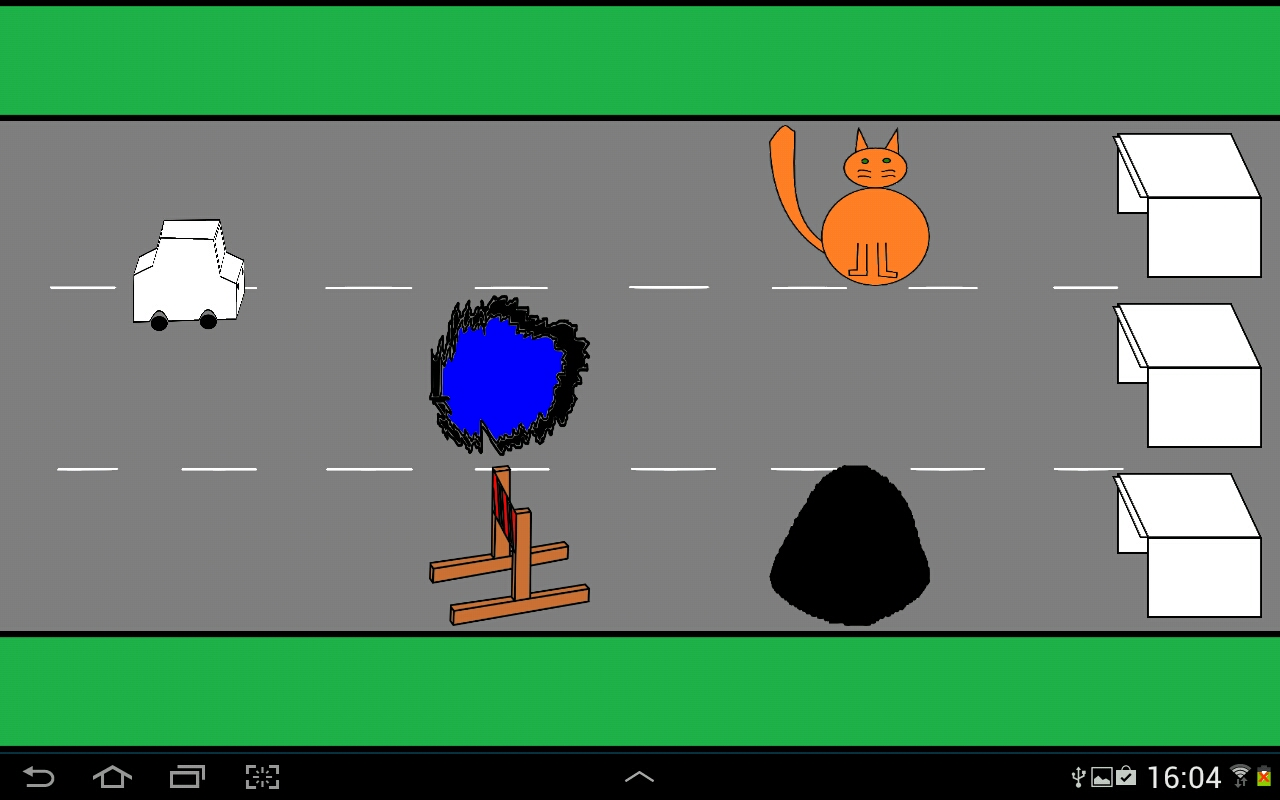
\includegraphics[width=.5\textwidth]{sprint1/cars_screenshot}
\caption{Screenshot from the 'Cars' app.}
\label{fig:cars_screenshot}
\end{figure}

Sound input is an important element of Cars, as it is used to control the car.
It was also a part of the game which did not work properly.
The car's movements did not correctly correspond to the voice input, seemingly causing the car to move at random, no matter what kind of pitch was used.

Using voice input based on pitch was an original requirement of the Cars project, worked out between the Cars group and the stakeholders.
Its intention was to solve a particular problem concerning some autists, not being able to control their pitch during speech.
Based on its importance and that it does not work, this would be a natural major focus point during the first sprint.

However, in the following two sections of this chapter, we will argue that there are two overall problems with trying to improve the already existing Cars project.
Firstly we will argue that it is very difficult to obtain frequency from sound input.
Secondly we will argue that it would be easier to completely reboot the Cars project, with new framework and structure, rather than continuing on the existing code and structure.

We will instead argue for using volume instead of pitch, after confirming its validity with the stakeholders.
Additionally we will propose a structure, based on the KiloBolt framework.
\newpage

\section{Obtaining frequency from sound}
The current method of controlling the player (the car) in Cars, is based on sound input.
When the game is running, voice input is continually recorded and analysed, in order to detect the pitch of the sound input, so that the direction in which to move the car can be decided.
The current method of analysing this is by using Fast Fourier's Transformation (FFT) and subsequently choosing the loudest frequency.

In this section we will briefly explain what sound is, in order to understand how to obtain certain characteristics of sound.
Based on this knowledge we will argue why it is difficult to obtain frequency from a sound input, especially sound input with human voice.
The technicalities in the section are based on \cite{music-and-computers}.

\subsection{Characteristics of sound}
Sound is a physical phenomenon which acts like a wave and therefore have the same characteristics as a wave.
So basically sound is a movement of air and the way we perceive sound is an interpretation of these movements.

Simply speaking, the volume (or loudness) of a sound, is the amplitude of the sound wave.
The pitch of a sound, how high/low we perceive it, is the frequency of the sound wave.
These two characteristics are independent, meaning that two sound waves with same frequency, but different amplitudes, will sound like the same pitch, but one being louder than the other.
An example can be seen in \cref{fig:samepitchdiffamp}.

\begin{figure}[h]
\centering
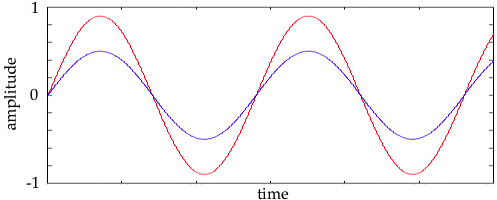
\includegraphics[width=.80\textwidth]{sprint1/samepitchdiffamp}
\caption{Two sound waves (represented as sine functions) with same frequency, but different amplitude.}
\label{fig:samepitchdiffamp}
\end{figure}

There is also a third characteristic, which is more abstract and not directly a physical attribute, namely, timbre.
Timbre is a composition of different sound waves (spectra), which makes up a specific sound (again, this is perceptual) and envelope (transients), which describe the different stages of a sound.

\subsection{Obtaining frequency}
Obtaining frequency is fairly simple, as it can read from a sound input interpreted as a wave (sine function).
However, some sounds are simpler than others in their composition of waves.
These simpler sounds could be considered ''cleaner'' than others, meaning they consist of only a single or very few waves, where it is easy to identify a primary amplitude and frequency.

Human speech, among other sounds, consists of multiple sound waves, each with varying amplitude and frequency.
In this case, it may be difficult to point out a single wave as the most important, and choose its frequency as the main frequency.
A comparison between frequency spectra can be seen in \cref{fig:frequency_spectra}.

\begin{figure}[h]
\centering
\begin{subfigure}[t]{.45\textwidth}
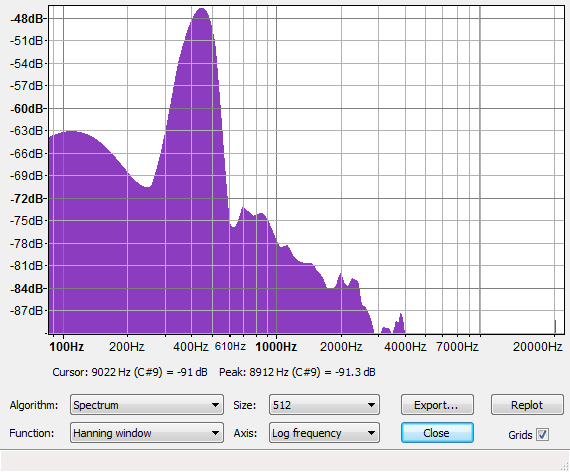
\includegraphics[width=\textwidth]{sprint1/spectrum_tonegenerator}
\caption{Frequency spectrum for a 440 Hz generated tone}
\end{subfigure}
\begin{subfigure}[t]{.45\textwidth}
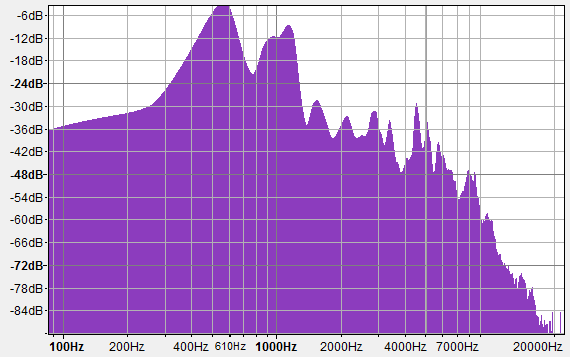
\includegraphics[width=\textwidth]{sprint1/spectrum_highpitchvoice}
\caption{Frequency spectrum for human voice input (in an attempt to reach high pitch)}
\end{subfigure}
\caption{Frequency analysis in Audacity}
\label{fig:frequency_spectra}
\end{figure}

\subsection{Using FFT}



\section{Redesigning Cars}
\section{Design Evaluation}
The original goal of the first sprint was to refactor the Cars project. 
After using a few weeks reading and changing the code it turned out to be more complicated than initially assumed.
The changes we made was small but required extensive work because of the lack of structure in the project.
It was decided that a total redesign of the application would be the better option.
Instead of spending a lot of time trying to understand and modify the code, a redesign would not only take shorter time but would also result in a better design.

The following sections will summarize the problems that made the task of refactoring the cars project near impossible.
\subsection{Inheritance}
It seems that the authors of the code are not familiar with the OOP term inheritance.
Inheritance in OOP is when you have a class based on an other class.
This is useful for code reuse.

An example of good use of inheritance is if we have a class called \textit{Vehicle}.
Which e.g. has a method \textit{ChangeOwner} and a field \textit{RegistrationNumber}.
We can then make a specialisation of \textit{Vehicle} e.g. called \textit{Car} and \textit{Truck}.
These two new classes can now also use the method and field there is in \textit{Vehicle}.
This means the code gets reused, instead of having it in both \textit{Car} and \textit{Truck} we have it only in \textit{Vehicle}.

An example from 'Cars' is the class \textit{GameObject} which is an empty super class to the following classes:

\begin{tabular}{ c  c }
\parbox{\textwidth/2}{
\begin{itemize}
\item Barricade
\item Bump
\item Car
\end{itemize}} &
\parbox{\textwidth/2}{
\begin{itemize}
\item Cat
\item Garage
\item Rock
\end{itemize}
}
\end{tabular}
The classes shown above all have a \textit{draw} method which are identical.
This is a classic example on a method which should have been in the super class.
If it would have been in the super class all its derived classes could have used the method.
This would then be good code reuse.
\subsection{Methods}
This paragraph will contain the general problems with the methods in the project 'Cars' and their usability.
\\
Understanding a method is difficult when it is big and has different operations.
One should instead split them up to small methods, for instance an operation per method.
\\
An example of an operation could be to fill a whole array with a certain number.
The code for this would be a for-loop filling an array with the number.
Instead of having the code in the method, where you then will use it, it is better to create a method for that and call it.
This in general makes the maintenance and refactoring of the code easier, because the code then has a higher readability.
\\
The \textit{Run} method\cref{abe} from 'Cars' from the class \textit{RecorderThread} is a classic example on a method which should be smaller.

\subsection{Object Oriented Design}
A problem throughout the code is that basic object oriented principles are not used or are not used properly. 
Classes do not have a clearly defined responsibility, and functionality is instead spread out on several classes. 
This breaks the concept of keeping high cohesion in object oriented design. 
Cohesion is a measure of how the responsibilities of a module are related. 
If the responsibilities are highly related, the module is said to have high cohesion.
An advantage of high cohesion is that it improves maintainability of the system, because changes in one module requires fewer changes in other modules. \stefan{source på cohesion (OOAD)?}

An example of low cohesion in the cars project is the \lstinline!Car! class(\cref{car_class}).
This class has the responsibility to draw itself, move itself according to pitch of the sound recorded by the microphone, calculate collisionboxes and determine if the car has collided with an obstacle and close the garage if the car has driven into the goal garage.

Another concept the existing code breaks is coupling.
Coupling is the number of  dependencies between modules.
It is desirable to keep this number as low as possible, known as having low coupling.
Low coupling has the advantage of making it easier to make changes in module, as they are not independent on each other.

When trying to read and understand the existing implementation of the control of the car by pitch, it turned out to be very hard.\stefan{possibly a reference to FFT analysis chapter}
Because the code responsible for handling the pitch is spread out on several classes, this relatively simple change becomes very complicated.
Another example is the responsibility for drawing objects which is on the individual object instead of using inheritance as described in \cref{sprint1_inheritance}. 
This makes it very hard to make consistent changes to the way objects are drawn.
\stefan{code examples?} 


\chapter{Sprint 2}

\chapter{Sprint 3}

\chapter{Sprint 4}

\chapter{Common Activities}

\chapter{Conclusion}
\input{content/conclusion.tex}

\chapter{Future Work}

\chapter{Reflections}

\appendix
% PART ******************************
\part[Appendix]{Appendix\\
	\begin{minipage}[c]{10cm}
	\centering
	\vspace{2cm}
	\normalsize{\textnormal{
		\textit{}
	}}
	\end{minipage}
}

\chapter{Code example: Run method from class RecorderThread}
\begin{lstlisting}[style=csharp,label=big_run_method, caption={Run method from the original Cars project.}]
@Override
public void run() {

System.out.println("recorderThread started");
AudioRecord recorder;
int p;
short[] audioData;
int bufferSize;
int Samplerate = 44100;
bufferSize=AudioRecord.getMinBufferSize(Samplerate,AudioFormat.CHANNEL_IN_MONO,
AudioFormat.ENCODING_PCM_16BIT)*2; //get the buffer size to use with this audio record  

recorder = new AudioRecord (AudioSource.MIC,Samplerate,AudioFormat.CHANNEL_IN_MONO,
AudioFormat.ENCODING_PCM_16BIT,bufferSize); //instantiate the AudioRecorder


recording=true; //variable to use start or stop recording
audioData = new short [bufferSize]; //short array that pcm data is put into.

while (recording) {  //loop while recording is needed
	if (recorder.getState()==android.media.AudioRecord.STATE_INITIALIZED){ // check to see if the recorder has initialized yet.
	}
	if (recorder.getRecordingState()==android.media.AudioRecord.RECORDSTATE_STOPPED){
	recorder.startRecording();  //check to see if the Recorder has stopped or is not recording, and make it record.
	}
	else {
	recorder.read(audioData,0,bufferSize); //read the PCM audio data into the audioData array
	double[] endAudioData = new double [bufferSize*2];                        
	//Now we need to decode the PCM data using the Zero Crossings Method
	//FFT fft1 = new FFT();
	short[] imgAudioData = new short [bufferSize];
	endAudioData = FFT.fft(audioData,imgAudioData, true);

	double[] magnitude = new double [bufferSize-1];
	int highestMagnitude = 0;
	for (p=2;p<(bufferSize-1)*2;p+=2){
	magnitude[p/2-1] = Math.sqrt(endAudioData[p]*endAudioData[p] + endAudioData[p+1]*endAudioData[p+1]);
	//System.out.println("magnitude = " + magnitude[p/2-1]);
	if (magnitude[p/2-1] > magnitude[highestMagnitude]){
	highestMagnitude = p/2-1;
	}
	}
	int i;
	double[] frequency = new double [bufferSize-1];  
	for (i=0 ; i<(bufferSize-1) ; i++){
	frequency[i] = ((i+1) * Samplerate/2) / (bufferSize/2);
	}

	double total = 0;
	double magnitudeTotal = 0;
	int start;
	if (highestMagnitude > 2) {
	start = -2;
	} else {
	start = 0;
	}
	int end;
	if (highestMagnitude + 2 < frequency.length) {
	end = 2;
	} else {
	end = 0;
	}
	for (i=start ; i<end ; i++){
	total += frequency[highestMagnitude+i]*magnitude[highestMagnitude+i];
	magnitudeTotal += magnitude[highestMagnitude+i];
	}
	double averageFreq = total/magnitudeTotal;
	if (averageFreq<=highestHumanPitch && magnitudeTotal>voiceSensetivity) {
	currentFrequency = (int) averageFreq;
	//System.out.println("average frequency = " + (int)averageFreq + " magnitude total = " + (int)magnitudeTotal);
	} else {
	currentFrequency = 0;
	}
	GameInfo.setCurrFreq(currentFrequency);
	}//else recorder started 
	} //while recording 

	if (recorder.getState()== android.media.AudioRecord.RECORDSTATE_RECORDING) recorder.stop(); //stop the recorder before ending the thread
	recorder.release(); //release the recorders resources
	recorder=null; //set the recorder to be garbage collected.    
}//run 
\end{lstlisting}

\bibliography{bibliography}
\bibliographystyle{plain}
\label{LastPage}
\end{document}
